%%%%%%%%%%%%%%%%%%%%%%%%%%%%%%%%%%%%%%%%%
% Beamer Presentation
% LaTeX Template
% Version 1.0 (10/11/12)
%
% This template has been downloaded from:
% http://www.LaTeXTemplates.com
%
% License:
% CC BY-NC-SA 3.0 (http://creativecommons.org/licenses/by-nc-sa/3.0/)
%
%%%%%%%%%%%%%%%%%%%%%%%%%%%%%%%%%%%%%%%%%

%----------------------------------------------------------------------------------------
%	PACKAGES AND THEMES
%----------------------------------------------------------------------------------------

\documentclass{beamer}

\mode<presentation> {

% The Beamer class comes with a number of default slide themes
% which change the colors and layouts of slides. Below this is a list
% of all the themes, uncomment each in turn to see what they look like.

%\usetheme{default}
%\usetheme{AnnArbor}
%\usetheme{Antibes}
%\usetheme{Bergen}
%\usetheme{Berkeley}
%\usetheme{Berlin}
%\usetheme{Boadilla}
\usetheme{CambridgeUS}
%\usetheme{Copenhagen}
%\usetheme{Darmstadt}
%\usetheme{Dresden}
%\usetheme{Frankfurt}
%\usetheme{Goettingen}
%\usetheme{Hannover}
%\usetheme{Ilmenau}
%\usetheme{JuanLesPins}
%\usetheme{Luebeck}
%\usetheme{Madrid}
%\usetheme{Malmoe}
%\usetheme{Marburg}
%\usetheme{Montpellier}
%\usetheme{PaloAlto}
%\usetheme{Pittsburgh}
%\usetheme{Rochester}
%\usetheme{Singapore}
%\usetheme{Szeged}
%\usetheme{Warsaw}

% As well as themes, the Beamer class has a number of color themes
% for any slide theme. Uncomment each of these in turn to see how it
% changes the colors of your current slide theme.

%\usecolortheme{albatross}
%\usecolortheme{beaver}
%\usecolortheme{beetle}
%\usecolortheme{crane}
%\usecolortheme{dolphin}
%\usecolortheme{dove}
%\usecolortheme{fly}
%\usecolortheme{lily}
%\usecolortheme{orchid}
%\usecolortheme{rose}
%\usecolortheme{seagull}
%\usecolortheme{seahorse}
%\usecolortheme{whale}
%\usecolortheme{wolverine}

%\setbeamertemplate{footline} % To remove the footer line in all slides uncomment this line
%\setbeamertemplate{footline}[page number] % To replace the footer line in all slides with a simple slide count uncomment this line

%\setbeamertemplate{navigation symbols}{} % To remove the navigation symbols from the bottom of all slides uncomment this line
}

\usepackage{graphicx} % Allows including images
\usepackage{booktabs} % Allows the use of \toprule, \midrule and \bottomrule in tables

\usepackage[utf8]{inputenc}

%----------------------------------------------------------------------------------------
%	TITLE PAGE
%----------------------------------------------------------------------------------------

\title[Regulamentação da Internet]{Regulamentação da Internet} % The short title appears at the bottom of every slide, the full title is only on the title page

\author{Rodrigo Magalhães dos Santos} % Your name

\institute[IPT] % Your institution as it will appear on the bottom of every slide, may be shorthand to save space
{
Instituto de Pesquisas Tecnológicas \\ Universidade de São Paulo \\ % Your institution for the title page
\medskip
\textit{rmagalhaes85@gmail.com} % Your email address
}
%\date{\today} % Date, can be changed to a custom date
\date{19/03/2014}

\begin{document}

\begin{frame}
\titlepage % Print the title page as the first slide
\end{frame}

\begin{frame}
\frametitle{Visão Geral}
\tableofcontents 
\end{frame}

%----------------------------------------------------------------------------------------
%	PRESENTATION SLIDES
%----------------------------------------------------------------------------------------

%------------------------------------------------
\section{Internet Regulation -- A Digital Cold War?} 
%------------------------------------------------

\begin{frame}
\huge{\centerline{Internet Regulation -- A Digital Cold War?}}
\normalsize{\centerline{(Regulamentação da Internet -- Uma Guerra Fria digital?)}}
\end{frame}

%------------------------------------------------

\begin{frame}
\frametitle{International Telecommunication Union (ITU)}
\begin{itemize}
\item Agência das Nações Unidas especializada em Tecnologias de Informação e Comunicação;
\item É uma organização marcadamente pragmática --- mesmo durante a Guerra Fria ela foi capaz de negociar o International Telecommunication Regulations (ITR), tratado que até hoje baliza as telecomunicações entre paises;
\end{itemize}
\end{frame}

%------------------------------------------------

\begin{frame}
\frametitle{International Telecommunication Union (ITU)}
\begin{itemize}
\item Tem realizado uma vasta gama de trabalhos úteis, como a alocação  de bandas de rádio-frequência, alocação de órbitas de satélites e estabelecimento de padrões;
\item Declara comprometimento com a missão de conectar as pessoas ao redor do mundo, estejam elas aonde estiverem;
\end{itemize}
\end{frame}

%------------------------------------------------

\begin{frame}
\frametitle{International Telecommunication Regulations (ITRs)}
\begin{itemize}
\item O tratado foi desenvolvimento em 1988;
\item Visa facilitar a interconexão e a interoperabilidade, em nível global, das telecomunicações através das fronteiras nacionais;
\item Até hoje não foi revisado;
\end{itemize}
\end{frame}

%------------------------------------------------

\begin{frame}
\frametitle{World Conference on International Telecommunications (WCIT)}
\begin{itemize}
\item Conferência organizada pela International Telecommunication Union (ITU);
\item Fórum para que Governos discutirem mudanças nos ITRs (International Telecommunications Regulations); 
\item A última edição ocorreu entre 3 e 14/12/2012 em Dubai, nos Emirados Árabes Unidos;
\end{itemize}
\end{frame}

%------------------------------------------------

\begin{frame}
\frametitle{World Conference on International Telecommunications (WCIT) -- Evolução}
\begin{itemize}
\item No início, a maioria dos paises estavam comprometidas com os formatos iniciais do Tratado;
\item No decorrer da Conferência, uma delegação formada por China, Rússia e outros países apresentou uma Proposta que, segundo a visão de muitos analistas, transformaria a Internet em um sistema de redes controladas pelos Governos Nacionais.
\item Terry Kramer, chefe da delegação dos Estados Unidos, alegou que não poderia assinar o Tratado em sua forma atual;
\end{itemize}
\end{frame}

%------------------------------------------------

\begin{frame}
\frametitle{World Conference on International Telecommunications (WCIT) -- Resultados}
\begin{itemize}
\item Após isso, outros países se uniram aos Estados Unidos. Dos 144 paises que tinham o direito de assinar o Tratado, apenas 89 o fizeram;
\item Estados Unidos alegam que o ITR não deveria deliberar a respeito da Internet tanto quanto o está fazendo. Segundo alegações;
\item \textbf{Exemplo:} a nova proposta ao ITR discutiria sobre a transmissão de Spam. Entretanto, proibir o Spam implica em definir quais tipos de conteúdo são permitidos e, consequentemente, haveria a possibilidade de ameaças à liberdade de expressão;
\end{itemize}
\end{frame}

%------------------------------------------------

\begin{frame}
\frametitle{Luta pela Liberdade ou Proteção de Interesses?}
\begin{itemize}
\item Supostamente, os Estados Unidos estariam preocupados com a liberdade da Internet;
\item Porém, deve-se considerar que boa parte do tráfego da Internet passa pelos Estados Unidos;
\item Além disso, os Estados Unidades abrigam vários dos principais players do mercado da Internet;
\item Em suma: o país é o que mais se beneficia com o \emph{status quo}.
\end{itemize}
\end{frame}

%------------------------------------------------

\begin{frame}
\frametitle{Impactos}
\begin{itemize}
\item No curto prazo, os impactos são limitados. Mesmo tendo sido assinado pela maioria dos países, o Tratado ainda precisa ser ratificado pelos estados-membro do ITU;
\item No médio prazo, os impactos são mais preocupantes: a ITU pode sair enfraquecida e, no longo prazo, isso pode prejudicar toda a vasta gama de regulações importantes realizada pela ITU (distribuição de faixas de rádio-frequência, órbitas de satélites, entre outros);
\end{itemize}
\end{frame}

%------------------------------------------------

\section{The Internet's Future Depends on Maintaining Its Free Spirit}

%------------------------------------------------

\begin{frame}
\huge{\centerline{The Internet's Future Depends}}
\huge{\centerline{on Maintaining Its Free Spirit}} 
\normalsize{\centerline{(O Futuro da Internet depende da manutenção de seu caráter livre.)}}
\end{frame}

%------------------------------------------------

\begin{frame}
\frametitle{A falta de regulamentação ao longo da história da Internet}
\begin{itemize}
\item Regulamentação é algo que contraria os fundamentos do sucesso da Internet;
\item No início, acreditava-se que a Internet não se espalharia pelo globo. Atualmente, a internet está presente até na Antártica;
\item As pesquisas que originaram a Internet começaram com o governo americano e depois passaram a ser suportadas pelo setor privado e outros governos;
\item Os padrões que fundamentam a Internet criaram uma plataforma que permitiram a qualquer um implementar uma rede e conectá-la a outras redes;
\end{itemize}
\end{frame}

%------------------------------------------------

\begin{frame}
\frametitle{Liberdade na Internet}
\begin{itemize}
\item Os modelos de interconexões que constituem a internet emergiram a partir de acordos bilaterais ou multilaterais entre diferentes partes;
\item A liberdade para a escolha de equipamentos, software, serviços e modelos de negócio foi crucial para o investimento em larga escala na Internet;
\item Os protocolos de rede que constituem a Internet são agnósticos em relação ao conteúdo que carregam $\rightarrow$ \textbf{Flexibilidade}
\end{itemize}
\end{frame}

%------------------------------------------------

\begin{frame}
\frametitle{O Protocolo IP no modelo de referência TCP/IP}
\begin{figure}
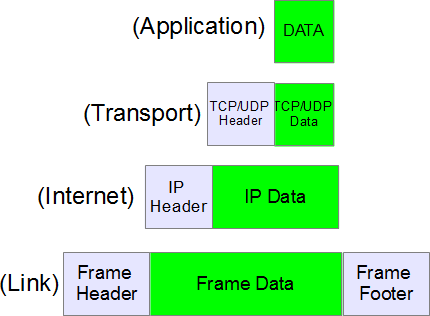
\includegraphics[width=0.6\linewidth]{ip-header-1.png}
\caption{Fonte: http://www.thegeekstuff.com/2012/03/ip-protocol-header/}
\end{figure}
\end{frame}

%------------------------------------------------

\begin{frame}
\frametitle{Instituições \emph{top down} vs \emph{bottom up}}
\begin{itemize}
\item Instituição \emph{top down}: criada a partir de leis, normas governamentais etc;
\item Instituição \emph{bottom up}: criada a partir da sociedade, costumes etc;
\item Um dos aspectos mais interessantes da evolução da internet é o surgimento de instituições bottom up visando manter e evoluir a capacidade da Internet;
\end{itemize}
\end{frame}

\begin{frame}
\frametitle{Instituições bottom up para a organização da Internet}
\begin{itemize}
\item Internet Configuration Control Board (ICCB) -- 1979: tornou-se a
\item Internet Activities Board -- 1984: tornou-se a
\item Internet Architecture Board -- 1992;
\item Internet Engineering Task Force -- 1986: desenvolve e promove padrões para a Internet; composta por voluntários;
\end{itemize}
\end{frame}

\begin{frame}
\frametitle{Conclusões}
\begin{itemize}
\item Os modelos de instituições bottom up e multi-stakeholder são mais apropriados para o desenvolvimento da Internet;
\item Tratados internacionais como o ITR são tipicamente compostos por acordos intergovernamentais $\rightarrow$ contramão do modelo bottom up;
\item Os governos possuem responsabilidades em relação aos seus cidadãos, mas as expectativas de todos os interessados devem ser ponderadas na elaboração de políticas;
\end{itemize}
\end{frame}

\section{Referências}
%------------------------------------------------

\begin{frame}
\frametitle{Referências}
\footnotesize{
\begin{thebibliography}{99} % Beamer does not support BibTeX so references must be inserted manually as below

\bibitem[L.S, 2012]{p1} L.S. (2012)
\newblock Internet Regulation -- A Digital Cold War?

\bibitem[Cerf, 2012]{p1} Vincent Cerf (2012)
\newblock The Internet's Future Depends on Maintaining Its Free Spirit

\bibitem[ITU]{p1} International Telecommunication Union
\newblock About ITU
\newblock \emph{Disponível em http://www.itu.int/en/about/Pages/default.aspx}

\end{thebibliography}
}
\end{frame}

%------------------------------------------------

\begin{frame}
\frametitle{Referências (cont.)}
\footnotesize{
\begin{thebibliography}{99} % Beamer does not support BibTeX so references must be inserted manually as below

\bibitem[Internet Society]{p1} Internet Society
\newblock World Conference on International Telecommunications (WCIT)
\newblock \emph{Disponível em http://www.internetsociety.org/wcit}

\bibitem[Internet Society]{p1} Internet Society
\newblock What are The ITRs?
\newblock \emph{Disponível em http://www.internetsociety.org/itr}

\bibitem[Institutions]{p1} William Easterly (2008)
\newblock Institutions: Top Down or Bottom Up?
\newblock \emph{Disponível em http://williameasterly.files.wordpress.com/2010/08/
55\_easterly\_institutionstopdownorbottomup\_prp.pdf}

\end{thebibliography}
}
\end{frame}

%------------------------------------------------

\begin{frame}
\Huge{\centerline{Dúvidas?}}
\end{frame}

%----------------------------------------------------------------------------------------

\begin{frame}
\Huge{\centerline{Fim}}
\end{frame}

%----------------------------------------------------------------------------------------

\end{document} 
